\documentclass[border=10pt]{standalone}

\usepackage{tikz}
\usepackage{tikzsymbols}
\usetikzlibrary{calc,patterns,shapes.geometric}

\def\centerarc[#1](#2)(#3:#4:#5){\draw[#1] ($(#2)+({#5*cos(#3)},{#5*sin(#3)})$) arc (#3:#4:#5);}

\begin{document}
	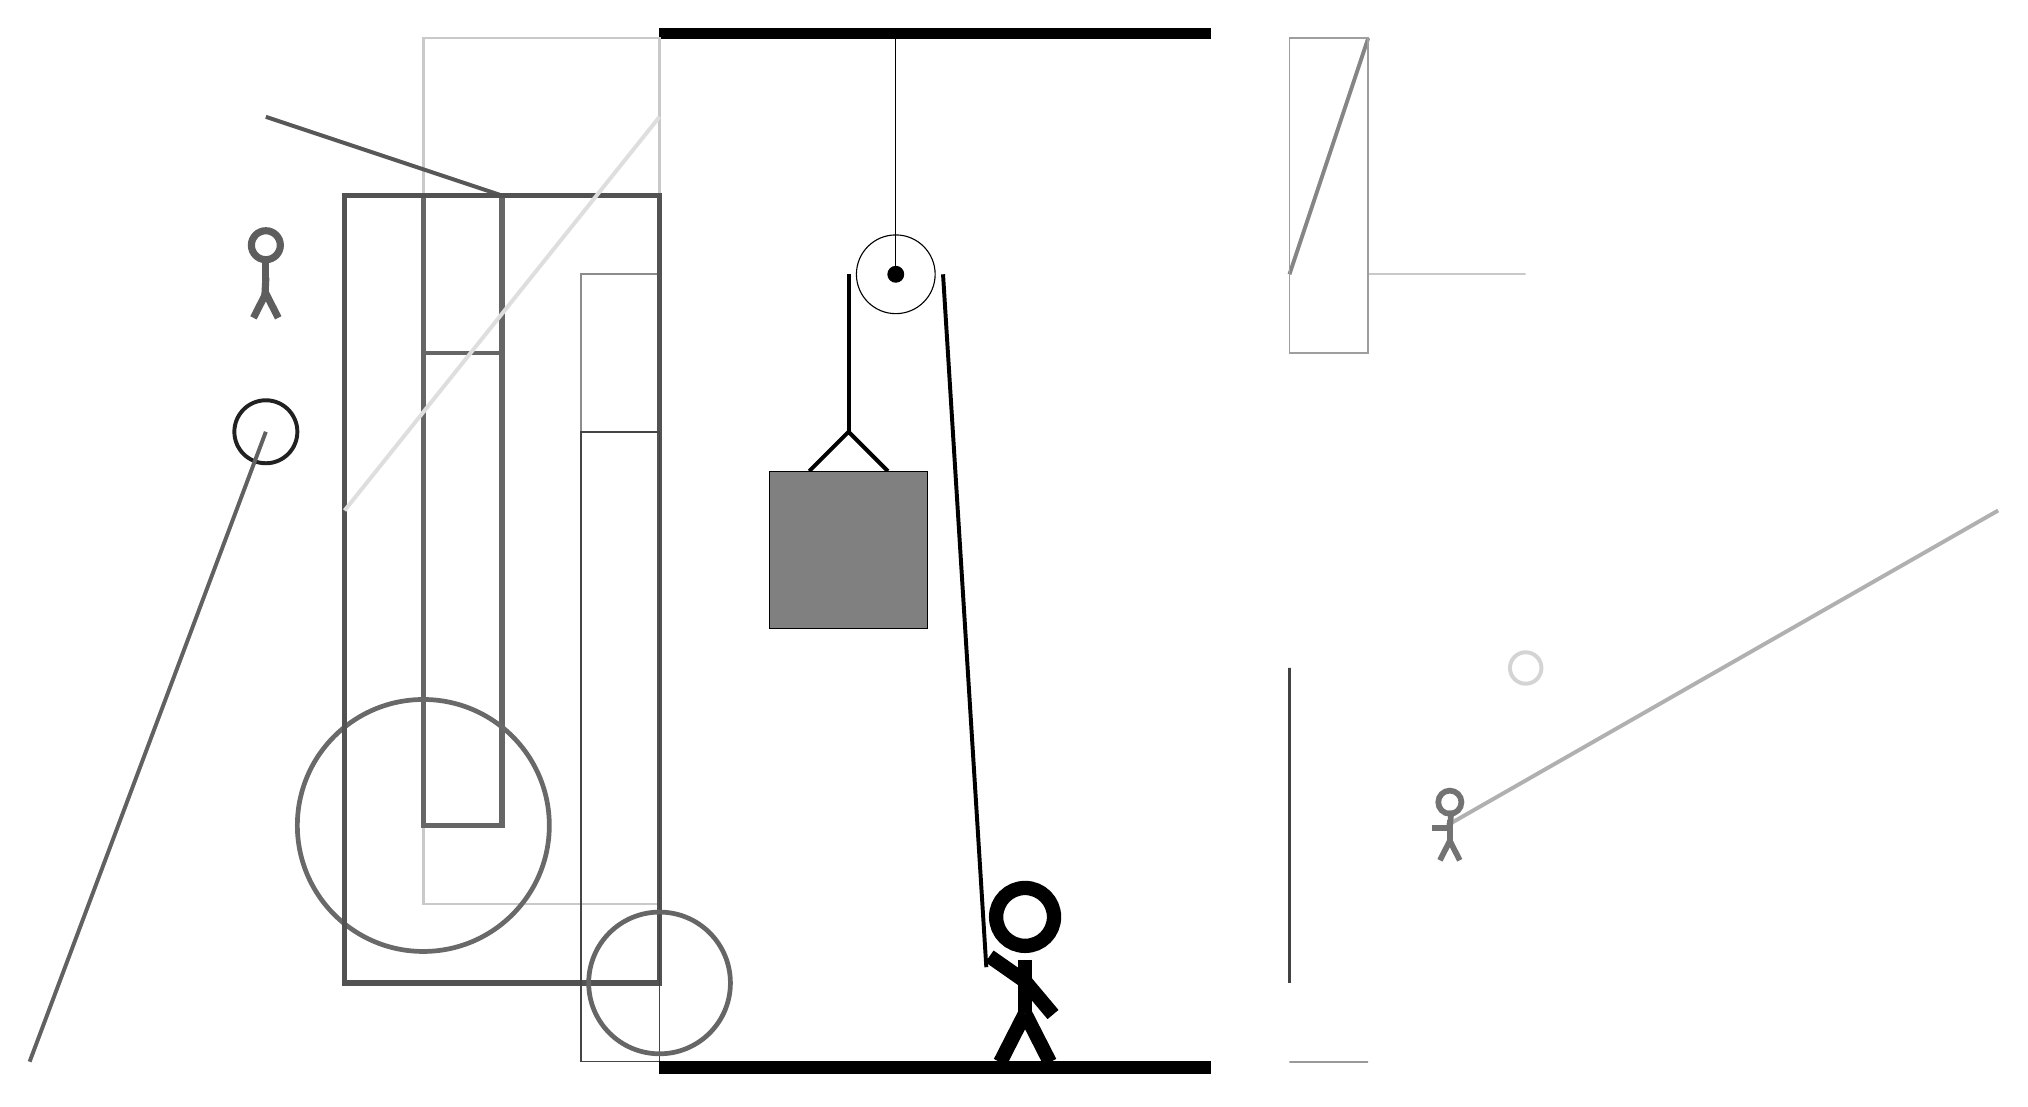
\begin{tikzpicture}
		%%%%% START %%%%%
		
		\draw[fill=black] (-2, 10) rectangle (5, 10.125);
		
		\draw (1, 7) circle (0.5);
		\draw[fill=black] (1, 7) circle (0.1);
		\draw (1, 10) -- (1, 7);
		
		\draw[line width=0.5mm] (-0.1, 4.5) -- (0.4, 5.0) -- (0.9, 4.5);
		\draw[fill=black!50] (-0.6, 4.5) rectangle (1.4, 2.5);
		
		\draw [line width=0.5mm, color=black!87](-7, 5) circle (0.4);
		
		\draw[line width=0.3mm, color=black!21] (-2, -1) rectangle (-5, 10);
		\draw[line width=0.3mm, color=black!21] (7, 7) rectangle (9, 7);
		\draw[line width=0.5mm, color=black!31](8, 0) -- (15, 4);
		
		\draw[line width=0.5mm, color=black!60] (-4, 6) rectangle (-5, 6);
		\draw[line width=0.3mm, color=black!40] (6, -3) rectangle (7, -3);
		
		\draw[line width=0.5mm, color=black!62](-7, 5) -- (-10, -3);
		\draw [line width=0.4mm, color=black!65](7, 9) circle (0.0);
		\node[line width=0.3mm, color=black!63] at (-7, 7) {\Strichmaxerl[5][87][90]};
		\draw[line width=0.3mm, color=black!45] (-2, 5) rectangle (-3, 7);
		
		\draw[line width=0.7mm, color=black!60] (-4, 0) rectangle (-5, 8);
		\draw[line width=0.5mm, color=black!48](7, 10) -- (6, 7);
		\draw[line width=0.2mm, color=black!38] (7, 6) rectangle (6, 10);
		
		\draw[line width=0.5mm, color=black!66](-4, 8) -- (-7, 9);
		\node[line width=0.4mm, color=black!55] at (8, 0) {\Strichmaxerl[4][0][85]};
		\draw [line width=0.6mm, color=black!59](-5, 0) circle (1.6);
		
		\draw[line width=0.7mm, color=black!68] (-2, -2) rectangle (-6, 8);
		
		\draw[line width=0.5mm, color=black!13](-2, 9) -- (-6, 4);
		\draw[line width=0.2mm, color=black!73] (-2, -3) rectangle (-3, 5);
		\draw [line width=0.6mm, color=black!60](-2, -2) circle (0.9);
		\draw [line width=0.5mm, color=black!17](9, 2) circle (0.2);
		\draw[line width=0.3mm, color=black!74] (6, -2) rectangle (6, 2);
		
		
		\draw[line width=0.5mm] (0.4, 7) -- (0.4, 5.0);
		\centerarc[line width=0.5mm](1, 7)(0:180:0.6);
		\draw[line width=0.5mm](1.6, 7) -- (2.15, -1.8);
		
		\node at (2.6, -1.9) {\Strichmaxerl[10][-35][-50]};
		
		\draw[fill=black] (-2, -3) rectangle (5, -3.15);
		
		%%%%% END %%%%%
	\end{tikzpicture}
\end{document}